\documentclass{ltjsarticle} %lualatex cs_jikken.texで作成 
\usepackage{mdframed}
\usepackage{graphicx}
\usepackage{float}
\usepackage{array}
\usepackage{tikz}
\usepackage{circuitikz}
\usetikzlibrary{automata, positioning, arrows}
\begin{document}

\thispagestyle{empty}
\begin{flushright}
{\large 実験実施日 2024年10月10日, 12日{\hspace{5cm}}} 
\end{flushright}

\vspace*{\fill}
\centering
{\Huge\bf コンピュータ科学実験b}
\vspace*{1cm}

{\huge\bf ハードウェア Raspberry Pi による制御}
\vspace*{\fill}

\vspace*{\fill}

\vspace*{\fill}

\begin{flushright}
{\large 学生番号: 102210017} \\ % 5cmの空白を作り、アンダーラインを引く
{\large 氏名: 安藤駿} \\
\end{flushright}

\clearpage

\addtocounter{page}{-1}
\raggedright
\setlength{\parindent}{1em}

\section{はじめに}
これまで様々なモノは個別に役割を果たしていたが, モノにセンサやアクチュエータを搭載し, インターネ
ットに接続可能とすることで, 現実世界の様々な情報収集, モノの遠隔制御, モノ同⼠の相互作⽤が可能とな
る. この考え⽅がIoT(Internet of Things)である. Raspberry Piを⽤いてIoTのデバイス管理を
体験, 学習する. Raspberry Piを⽤いたLED, スイッチ, ステッピングモータの制御を⾏う.


\section{課題2-1 単⼀LED(Light Emitting Diode)の点滅}

\subsection{目的・概要}
Raspberry Pi を⽤いてLED1個の点滅を⾏う. Raspberry PiとLEDを接続し, Raspberry Pi上でコー
ドを実⾏してLEDの点滅制御を⾏う. 

\subsection{必要な部品}

\subsubsection{Raspberry Piとその他部品}
• Raspberry Pi 3 model B+

• Micro SDカード(Raspberry Pi OS 書き込み済み)

• HDMIケーブル

• Micro USB電源ケーブル

• モニタ

実験室のモニタと自宅のモニタを使用した.

• USBキーボード

使用する製品は, SANWA社のSKB-KG3WNである. シリアル番号は, 20200500196である. 

• USBマウス

使用する製品は, ELECOM社のM-K6URBK/RSである. シリアル番号は, 1203314Cである. 


\subsubsection{ブレッドボード}
ブレッドボードは電⼦回路の試作に使⽤される. 電⼦部品の端⼦を差し込む⽳が多数存在し, それぞれの⽳
に差し込んだ端⼦が接続される.この接続関係を考慮して部品を配置することで, はんだ
付けを⾏うことなく電⼦回路を組むことができる.

\subsubsection{GPIOブレッドボード接続ケーブル}
Raspberry Pi の GPIOをブレッドボードへ接続することで, 部品の配線が容易となる.

\subsubsection{抵抗内蔵型LED}
⻑⾜側に抵抗が内蔵されている.

\subsection{実験方法}

\subsubsection{Raspberry Piの起動}
Raspberry Pi と液晶ディスプレイを HDMI ケーブルで接続した. 
Raspberry PiのUSB端⼦にキーボードとマウスを接続した.
Micro SD カードスロットにMicro SDカードを挿⼊した.
その後, Micro USB電源ケーブルをRaspberry Piに接続した.
このときの状況を, 図\ref{fig:raspi}に示す. 

\begin{figure}[H] % 画像を挿入する環境を開始
  \centering
  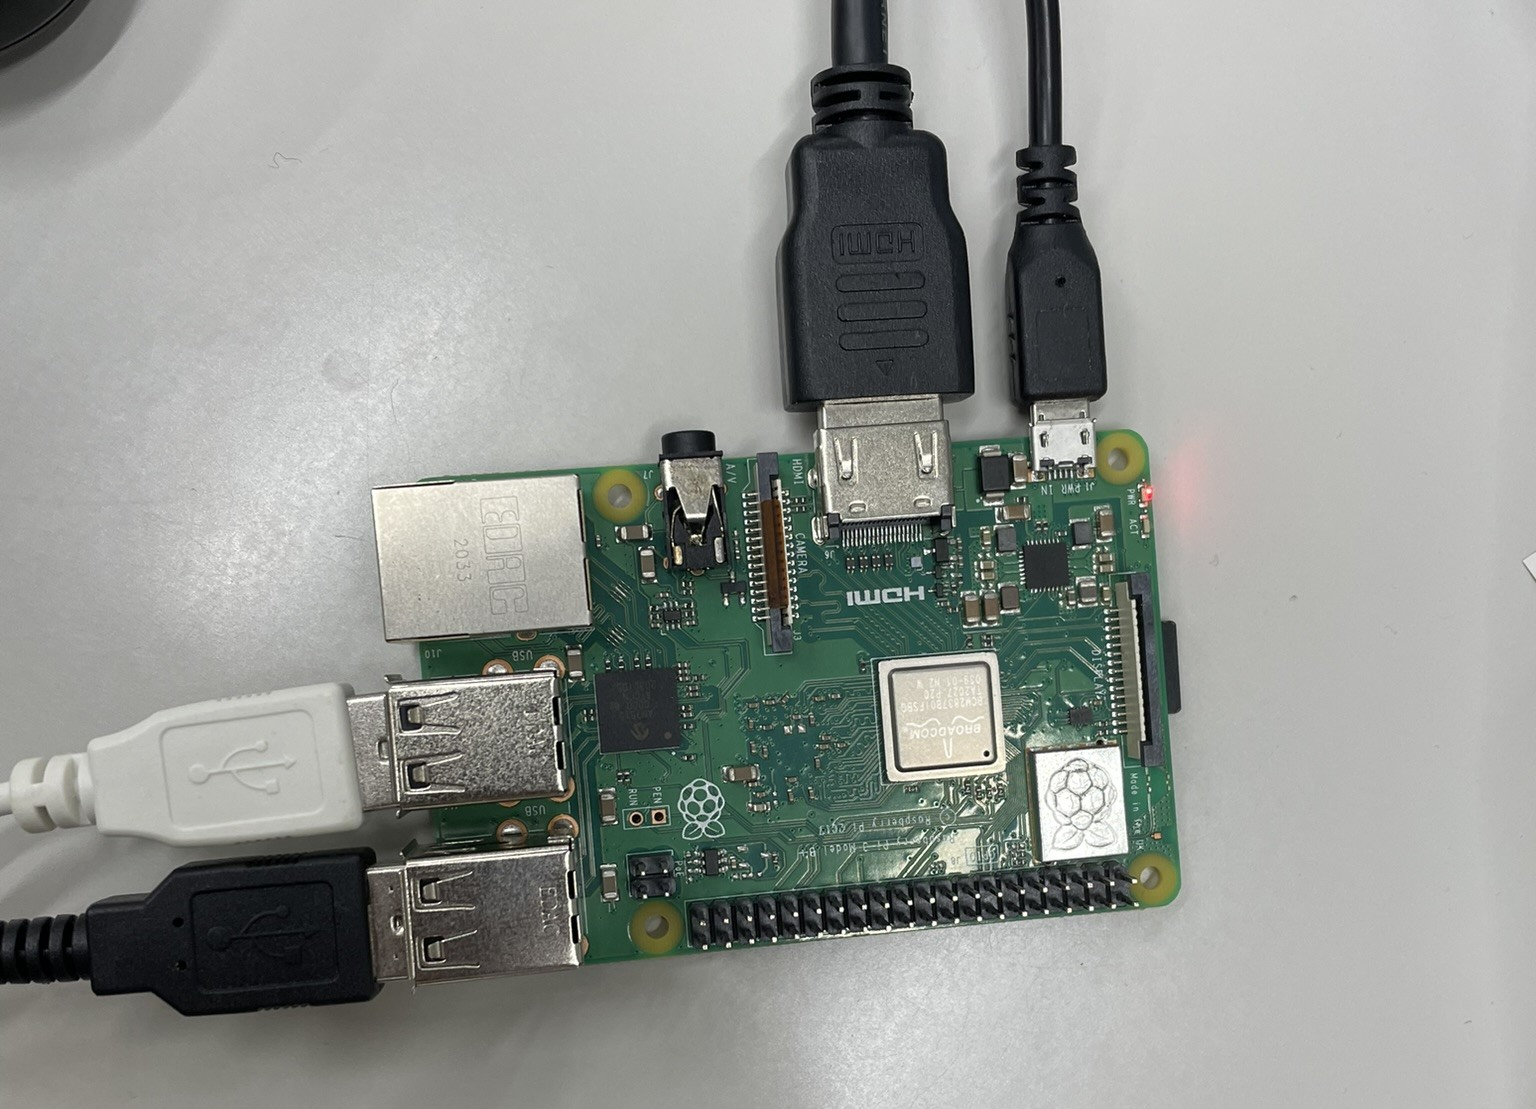
\includegraphics[width=0.5\textwidth]{raspi.JPEG} % 画像を挿入、幅をページ幅に合わせる
  \caption{ケーブル類を接続したRaspberry Pi} % キャプションを追加
  \label{fig:raspi} % ラベルを追加
\end{figure}

\subsubsection{OSのインストールと初期設定}
countryをJapan, timeをTokyoに設定した. usernameとpasswordを設定した. その後, 実験室内のwifiに接続した.
また, ソフトウェアのアップデートは行わなかった. ブラウザにfirefoxを選択した. そして, リスタートをした.

\subsubsection{⽇付の確認と設定}
ターミナルから「date」を入力し, 日時を確認した. 
その後,  「sudo date 101014052024」より, 正しい日時を設定した.

\subsubsection{Raspberry Pi のリモートログイン(SSH)設定}
「sudo raspi-config」より, 設定画面を開き, Interfacing Options, SSHを選び, 
SSH serverを有効にした. その後, hostnameを選択し, 「jikken-102210017」とした.
sudo rebootより, 再起動した.

自分のコンピュータから「shun@jikken-102210017.local」より, リモート接続を行った.


\subsubsection{ 単⼀LED (Light Emitting Diode)の点滅}
GPIOブレッドボード接続ケーブルをブレッドボードとRaspberry PiのGPIO端⼦に接続した. 
図\ref{fig:fig2-1}の回路図ように, GPIO4とGNDにLEDを接続した. 
本実験で⽤いるLEDは⻑⾜側に抵抗が内蔵されているので, ⻑⾜側をGPIOへ, 短⾜側をGNDへ接続した.

Raspberry PiによるLED点滅制御コード2-1.pyを作成した. これを, 図\ref{fig:2-1py}に示す.

その後, 2-1.pyをRaspberry Pi上で実行した.  

\begin{figure}[H] % 画像を挿入する環境を開始
  \centering
  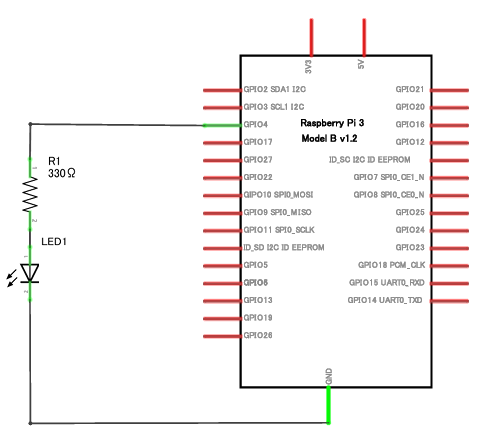
\includegraphics[width=0.5\textwidth]{fig2-1.png} % 画像を挿入、幅をページ幅に合わせる
  \caption{Raspberry Pi と LED1 個を接続する回路図} % キャプションを追加
  \label{fig:fig2-1} % ラベルを追加
\end{figure}

\begin{mdframed}
  \begin{verbatim}
    from gpiozero import OutputDevice
    import time
    # LED接続GPIO端⼦番号  
    LED_PIN = 4
    # LED⽤の出⼒端⼦を⽣成する
    led = OutputDevice(LED_PIN)
    while True:
        # LED接続端⼦をHighにする
        led.on()
        time.sleep(1)
        # LED接続端⼦をLowにする
        led.off()
        time.sleep(1)	
  \end{verbatim}
  \end{mdframed}
  \begin{figure}[H]
  \caption{2-1.py}
  \label{fig:2-1py}
  \end{figure}


\subsection{実験結果}

2-1.pyを実行した結果, 接続したLEDが点滅した.
この時の状況を, 図\ref{fig:raspi2-1}に示す.

\begin{figure}[H] % 画像を挿入する環境を開始
  \centering
  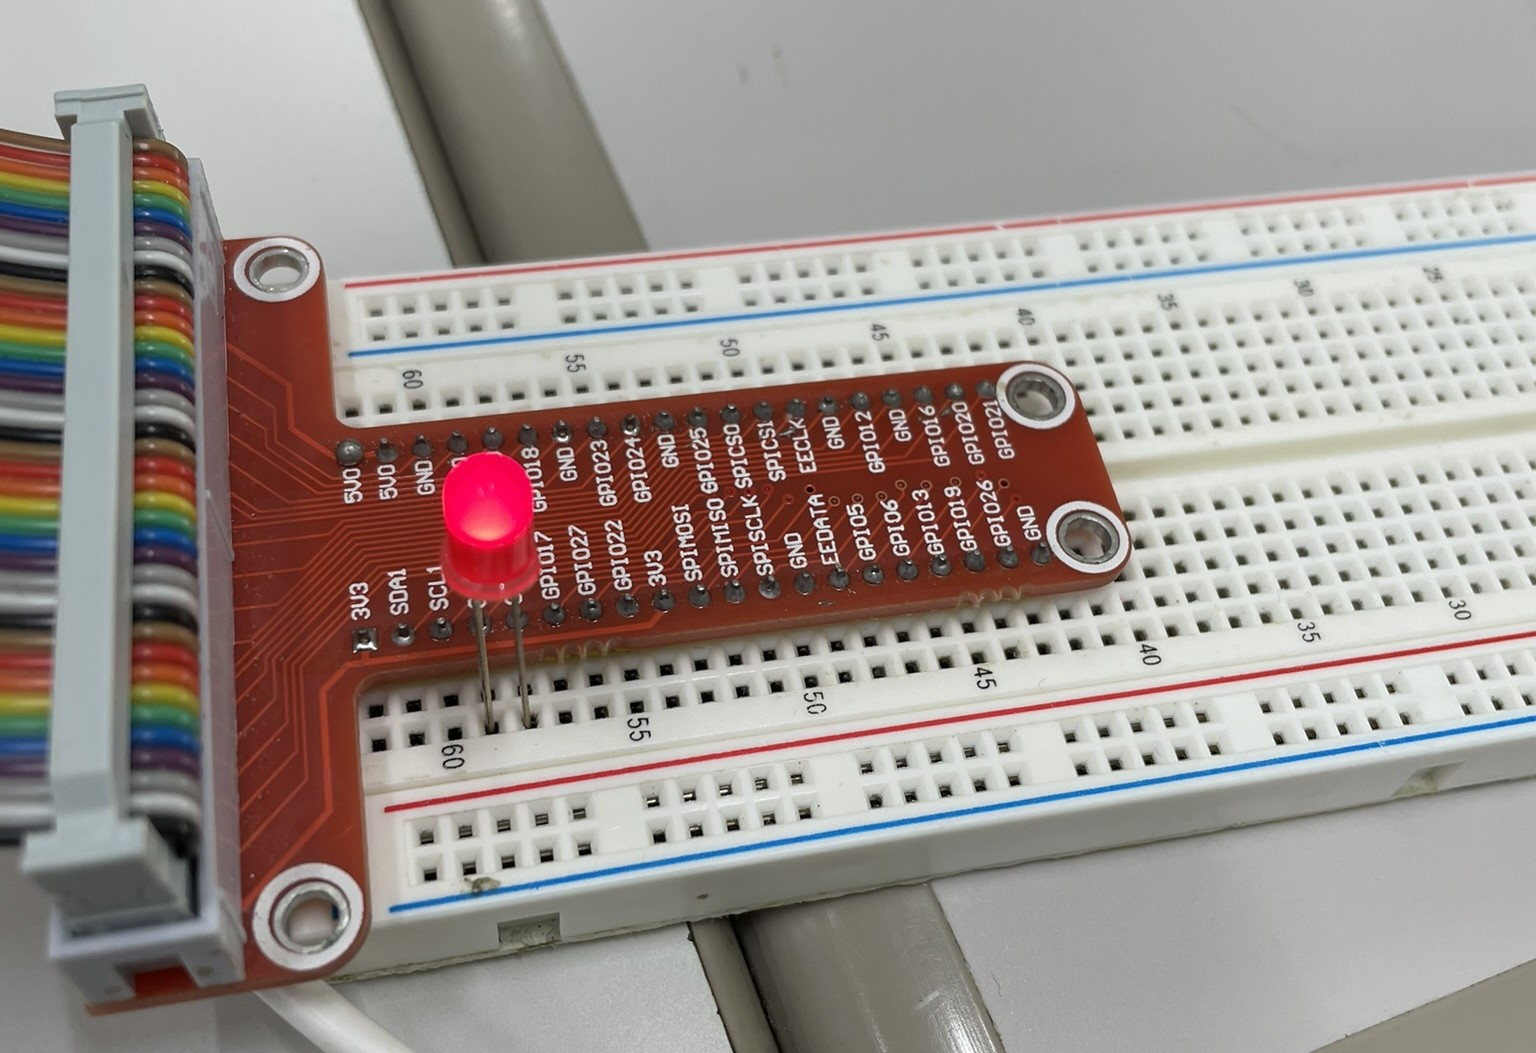
\includegraphics[width=0.5\textwidth]{raspi2-1.JPEG} % 画像を挿入、幅をページ幅に合わせる
  \caption{LED点滅の様子} % キャプションを追加
  \label{fig:raspi2-1} % ラベルを追加
\end{figure}

\subsection{考察}

LEDの点滅が1秒ごとだったのは,  time.sleep(1)でLEDがonとoffにされているからだと考えた. 


\section{課題2-2 単⼀スイッチの状態読み取り}

\subsection{目的・概要}
Raspberry Pi を⽤いて押しボタンスイッチ1個の状態読み取りを⾏う. 
押しボタンスイッチを使⽤する. 

\subsection{必要な部品}

\subsubsection{課題2-1と同じ部品}
Raspberry Pi 3 model B+, Micro SDカード
, HDMIケーブル, Micro USB電源ケーブル
, モニタ, USBキーボード, USBマウス
ブレッドボード, GPIOブレッドボード接続ケーブルは, 
課題2-1と同じものを使用する.

\subsubsection{押しボタンスイッチ}
2種類の端⼦を持ち, ボタンが押された間は2端⼦が導通状態, ボタンが押され
ていない間は解放状態となる.

\subsubsection{抵抗(1kΩ)}
金属皮膜抵抗1kΩ

\subsubsection{配線ケーブル}
オス-オスを使用した.

\subsection{実験方法}

図\ref{fig:fig2-2}の回路図ように, GPIO17とGNDの間に抵抗と押しボタンスイッチを配置した.
このときの状況を, 図\ref{fig:raspi2-2}に示す.

Raspberry Piによる押しボタンスイッチ読み取りコード2-2.pyを作成した. これを, 図\ref{fig:2-2py}に示す.
その後, 2-2.pyをRaspberry Pi上で実行し, スイッチを押したり離したりした.   

\begin{figure}[H] % 画像を挿入する環境を開始
  \centering
  \begin{minipage}{0.45\textwidth} % 1つ目の画像の幅をページの45%に設定
    \centering
    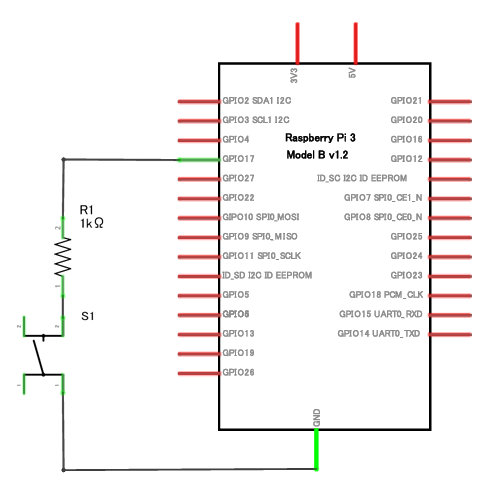
\includegraphics[width=\textwidth]{fig2-2.png} % 画像を挿入、幅をminipage幅に合わせる
    \caption{Raspberry Pi とスイッチ1個を接続する回路図} % キャプションを追加
    \label{fig:fig2-2} % ラベルを追加
  \end{minipage}
  \hfill % 画像の間にスペースを追加
  \begin{minipage}{0.45\textwidth} % 2つ目の画像の幅をページの45%に設定
    \centering
    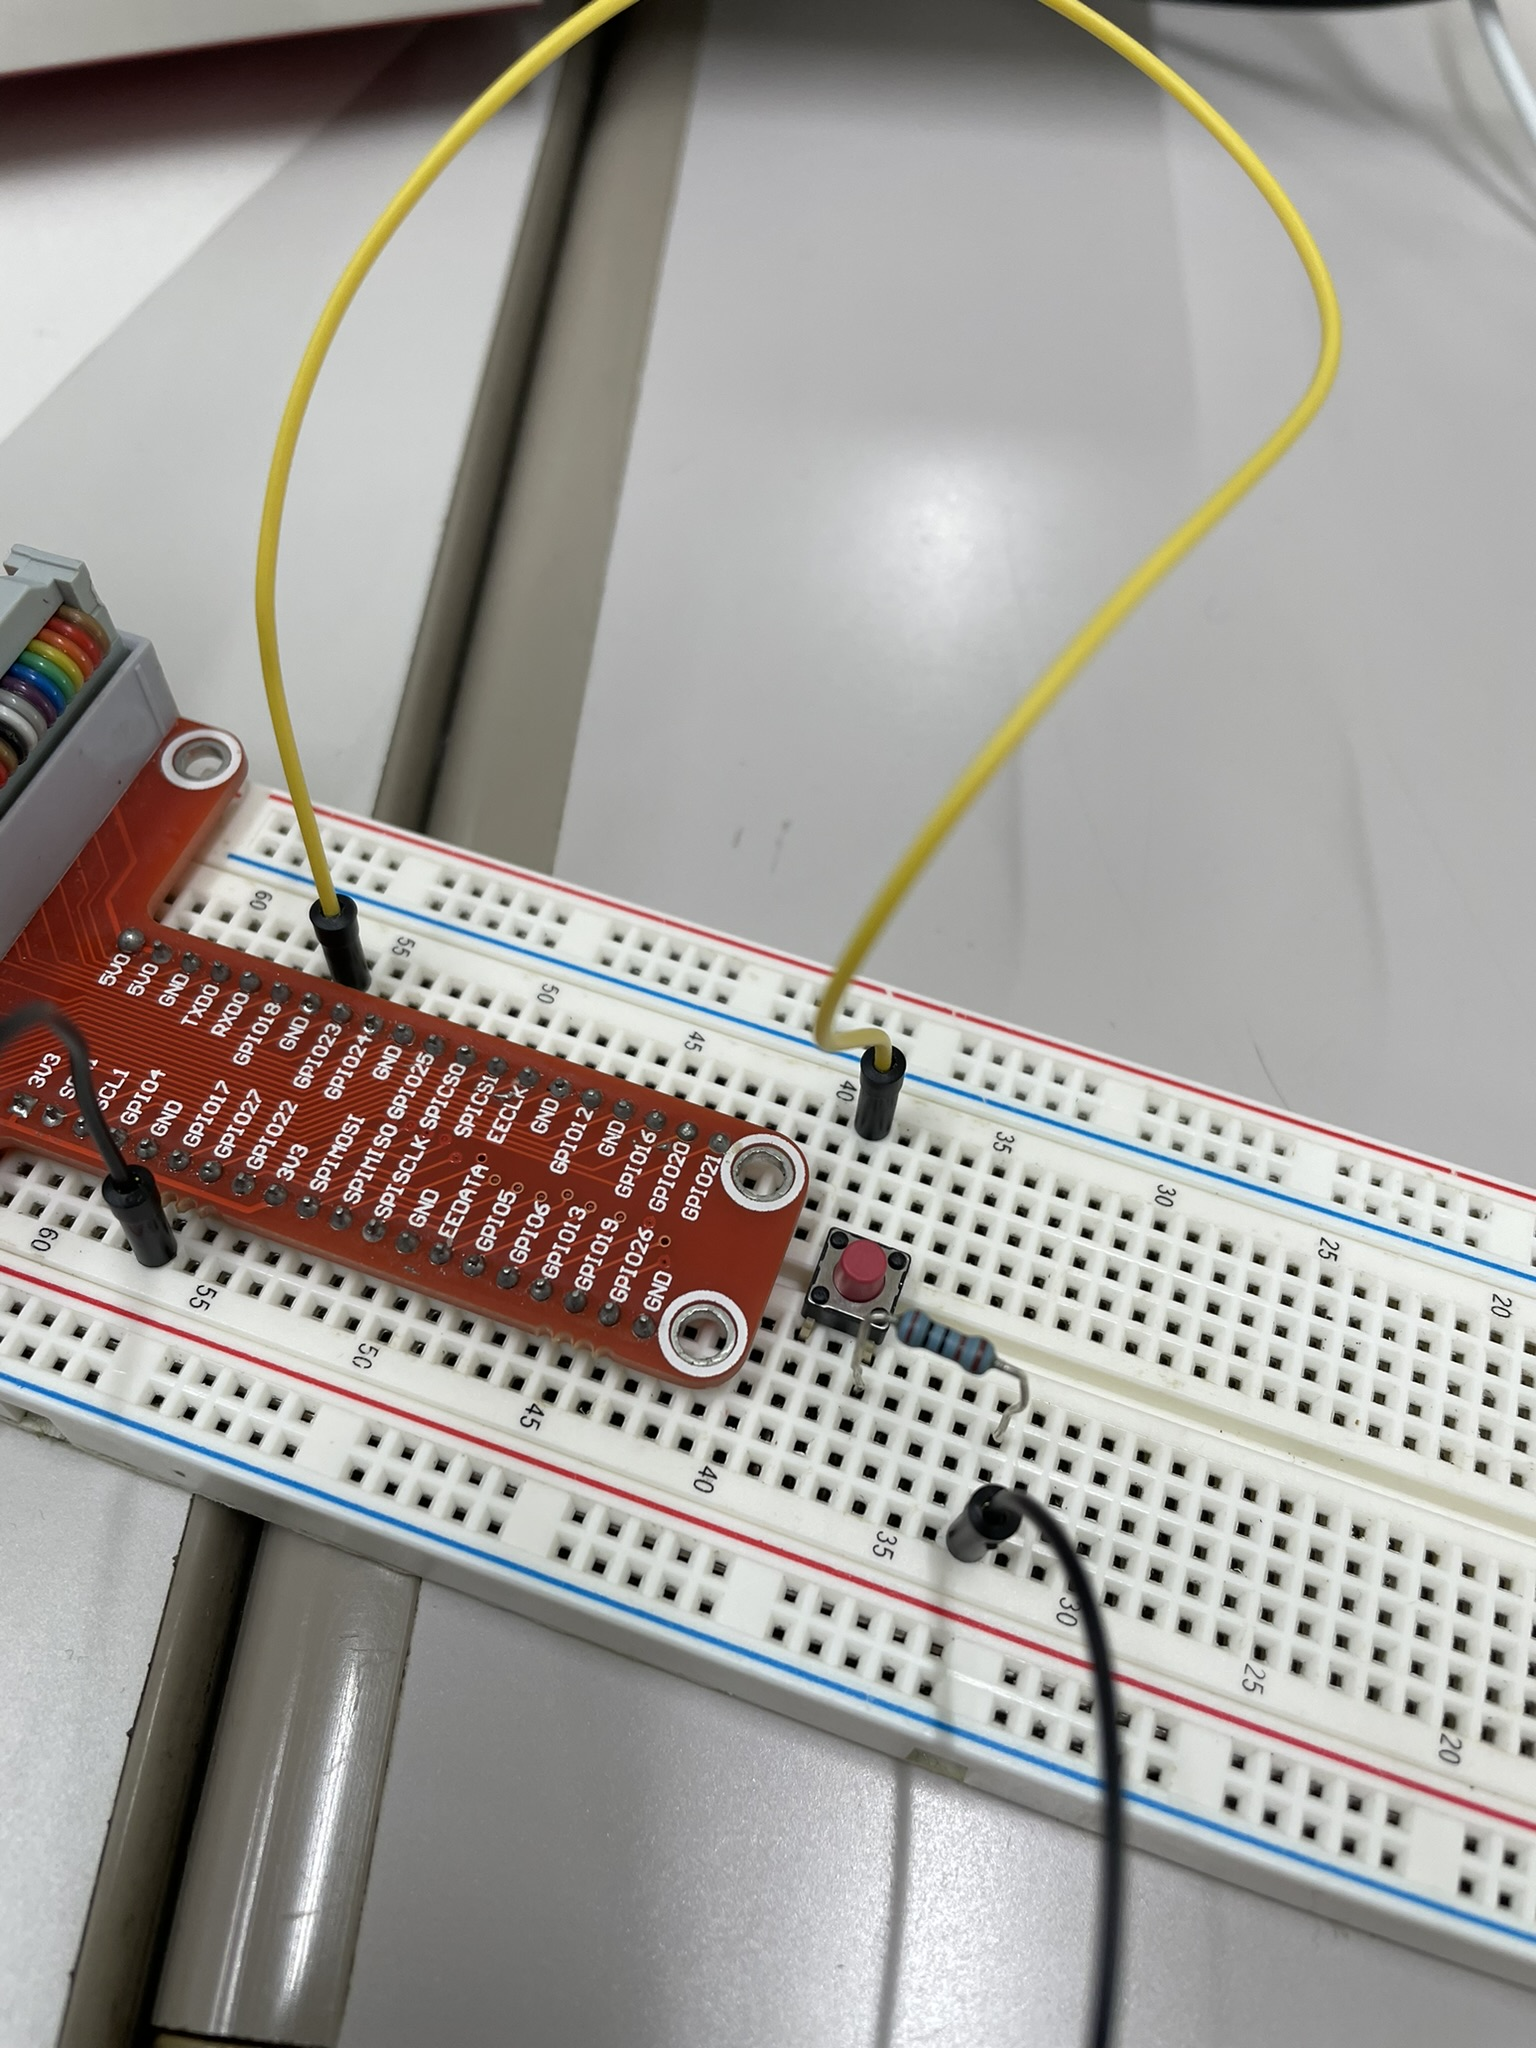
\includegraphics[width=\textwidth]{raspi2-2.JPEG} % 2つ目の画像を挿入
    \caption{課題2-2配線状況} % キャプションを追加
    \label{fig:raspi2-2} % ラベルを追加
  \end{minipage}
\end{figure}

\begin{mdframed}
  \begin{verbatim}
    from gpiozero import InputDevice
    import time

    # スイッチ接続GPIO端⼦番号
    SW_PIN = 17

    # スイッチ⽤にプルアップモードで⼊⼒端⼦を⽣成する
    switch = InputDevice(SW_PIN, pull_up=True)

    while True:
        # スイッチ接続端⼦の状態読み取り
        if switch.value == 1: # 押されていれば1(True)
            print("Switch on")
        else:
            print("Switch off")
        time.sleep(0.5)	
  \end{verbatim}
  \end{mdframed}
  \begin{figure}[H]
  \caption{2-2.py}
  \label{fig:2-2py}
  \end{figure}


\subsection{実験結果}

2-2.pyを実行した結果, switch on と switch offの出力がされた.
この時の状況を, 図\ref{fig:result2-2}に示す.

\begin{figure}[H] % 画像を挿入する環境を開始
  \centering
  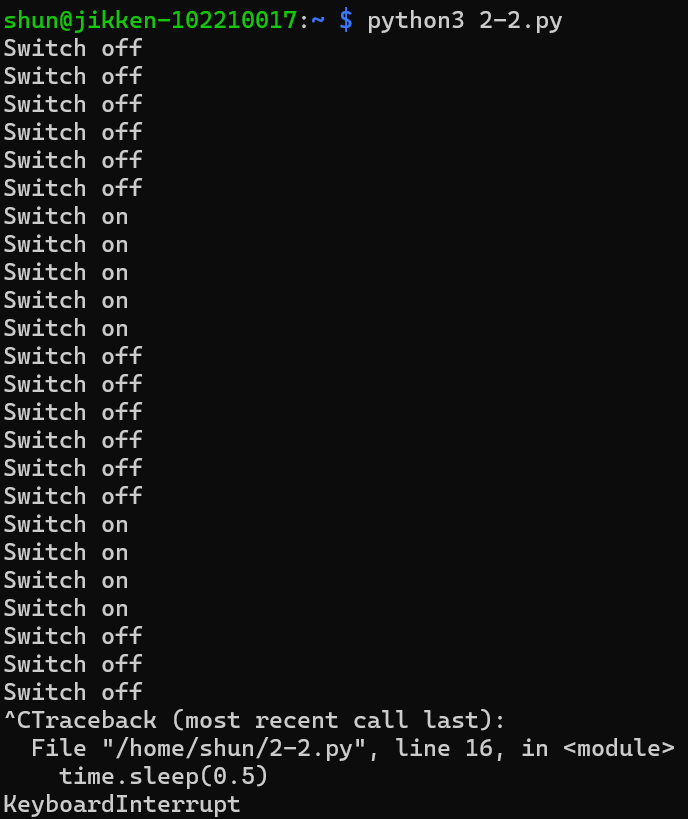
\includegraphics[width=0.5\textwidth]{result2-2.png} % 画像を挿入、幅をページ幅に合わせる
  \caption{スイッチを押した結果} % キャプションを追加
  \label{fig:result2-2} % ラベルを追加
\end{figure}

\subsection{考察}
スイッチが反応するのが0.5秒ごとだったのは, コードの最終行のsleep.time(0.5)のためであると考えられる. 
これによって, 連続でスイッチが押されたように反応することを防いでいると考えた. 


\section{課題2-3 複数LEDとスイッチの制御}

\subsection{目的・概要}
Raspberry Pi を⽤いて複数の LED とスイッチの制御を⾏う. 

\subsection{必要な部品}

\subsubsection{課題2-1, 2-2と同じ部品}
Raspberry Pi 3 model B+, Micro SDカード
, HDMIケーブル, Micro USB電源ケーブル
, モニタ, USBキーボード, USBマウス
ブレッドボード, GPIOブレッドボード接続ケーブル, 抵抗内蔵LED, 押しボタンスイッチ, 抵抗
, 配線ケーブルは課題2-1, 2-2と同じものを使用する. 



\subsection{実験方法}

表\ref{tab:tab2-3}のように, LEDと抵抗, 押しボタンスイッチを配置した.
このときの状況を, 図\ref{fig:raspi2-3}に示す. 

\begin{table}[H] % ここで[h]は表の位置をこの場所にすることを指定します
  \centering % 表を中央に配置
  \caption{回路の接続方法}
  \begin{tabular}{|c|c|c|} 
  \hline % 上の横線
  接続する部品 & GPIO端子の接続1 & GPIO端子の接続2 \\ \hline % 行の内容と行間の横線
  LED1 & GPIO4  & GND \\ \hline
  LED2 & GPIO17 & GND \\ \hline
  LED3 & GPIO27 & GND \\ \hline
  LED4 & GPIO22 & GND \\ \hline
  抵抗とSWITCH1 & GPIO5 & GND \\ \hline
  抵抗とSWITCH2 & GPIO6 & GND \\ \hline

  \end{tabular}
  \label{tab:tab2-3} % 表を参照するためのラベル
\end{table}

Raspberry Piによる複数LEDとスイッチの制御コード2-3.pyを作成した. これを, 図\ref{fig:2-3py}に示す.
その後, 2-3.pyをRaspberry Pi上で実行し, 二つのスイッチを押したり離したりした.

\begin{figure}[H] % 画像を挿入する環境を開始
  \centering
  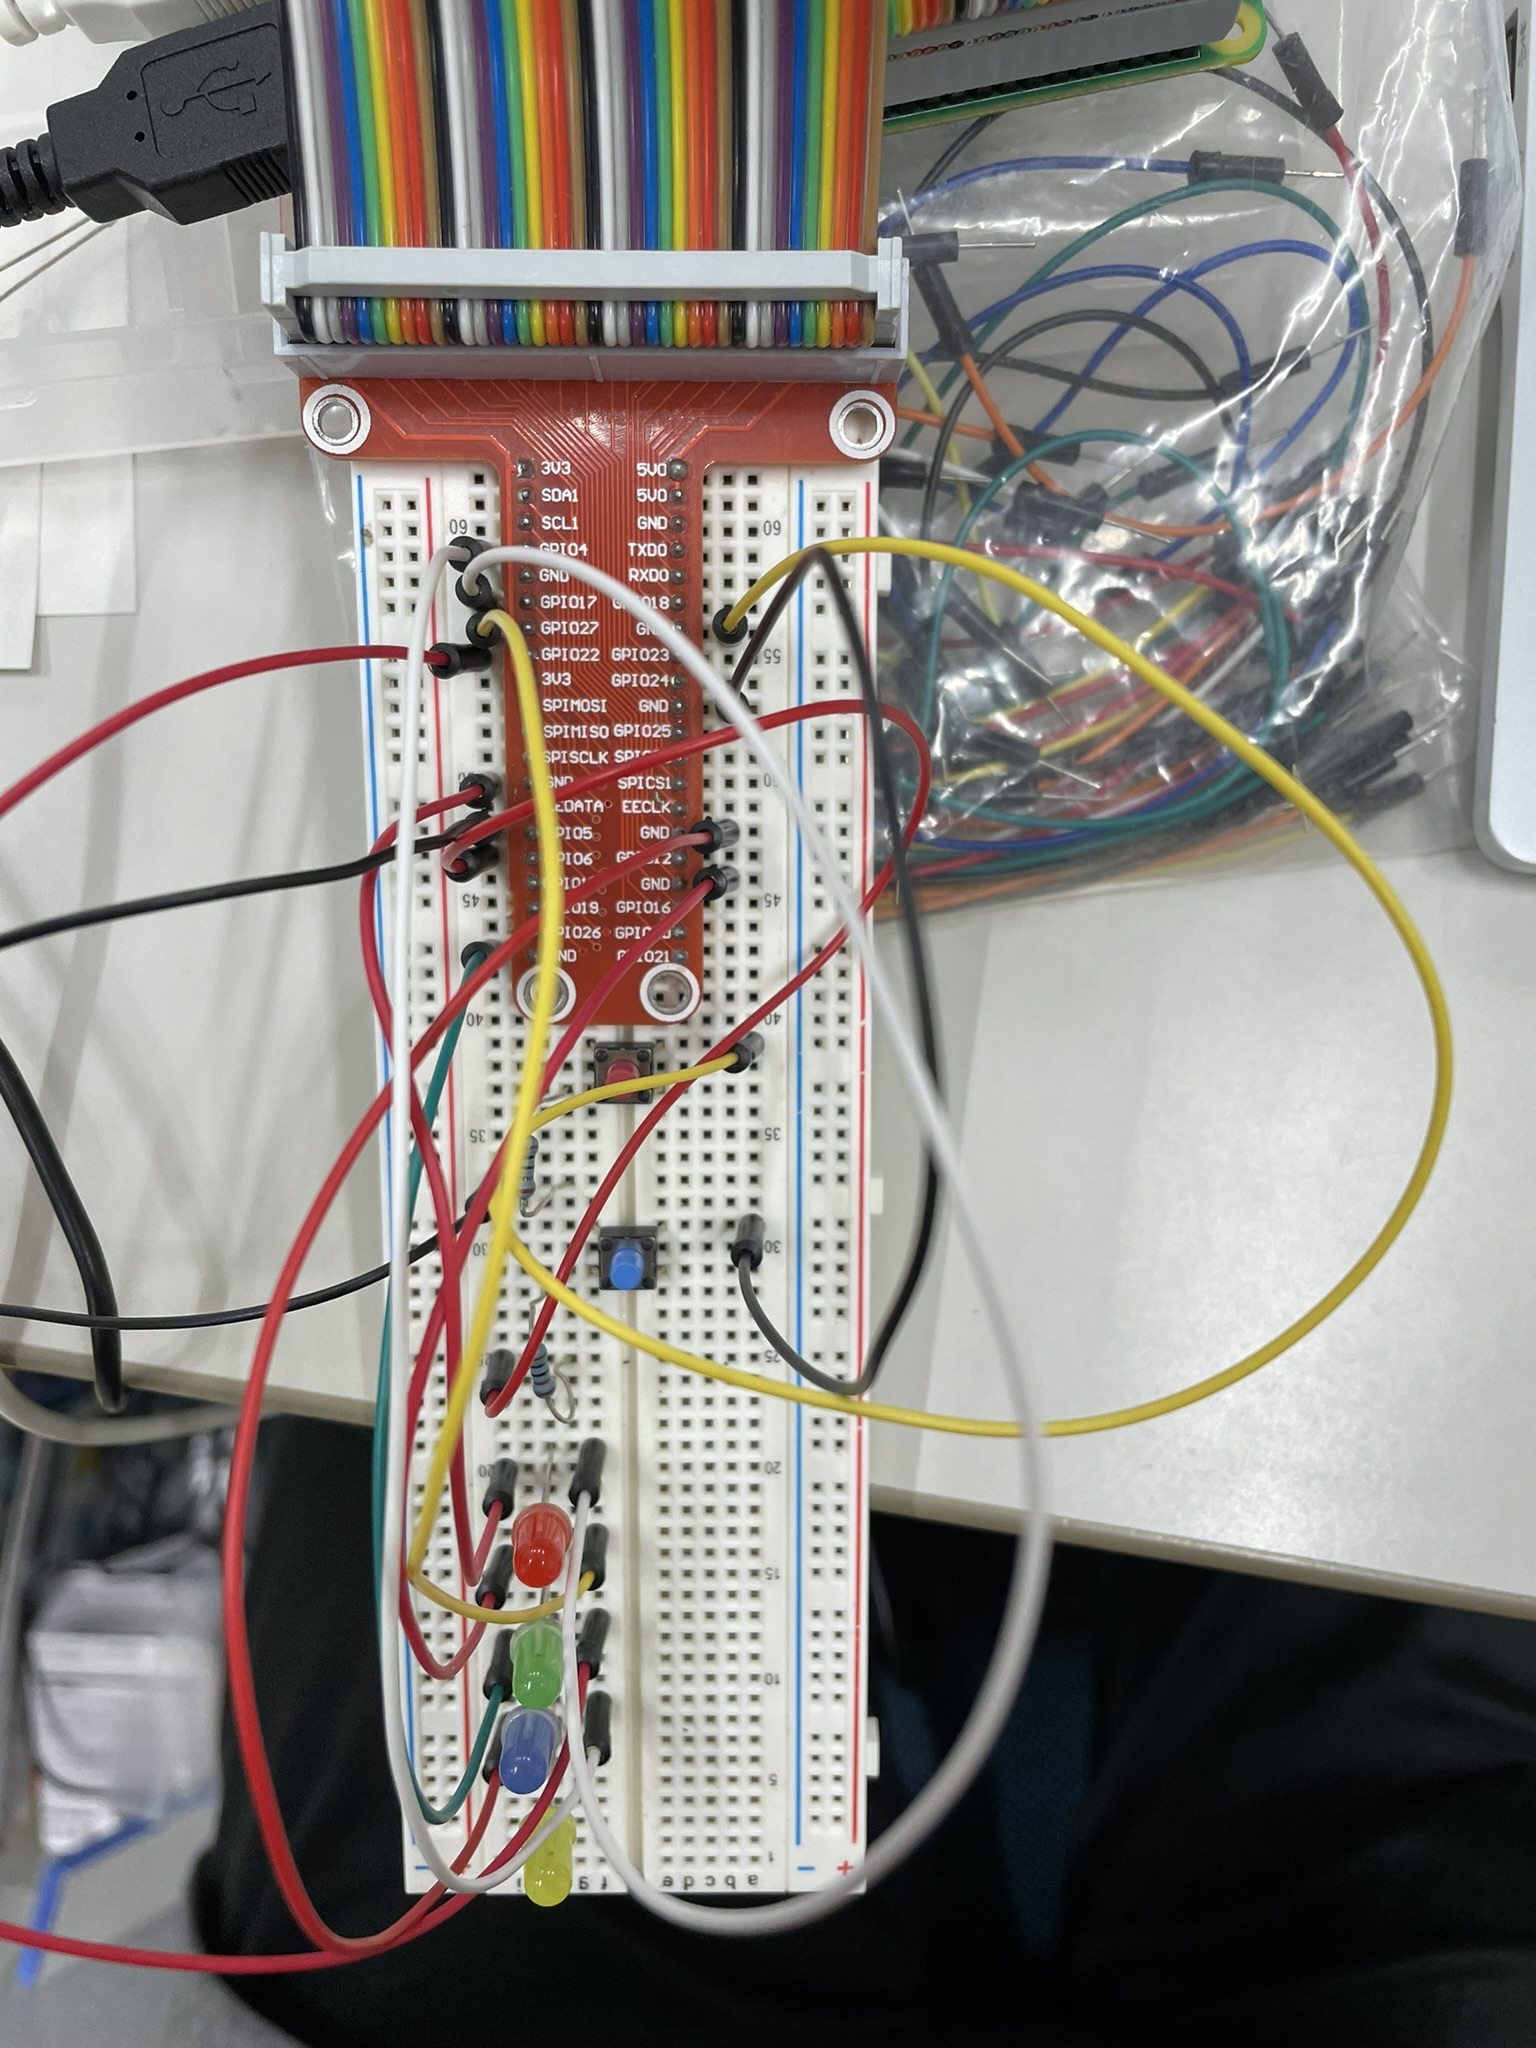
\includegraphics[width=0.5\textwidth]{raspi2-3.JPEG} % 画像を挿入、幅をページ幅に合わせる
  \caption{課題2-3の配線状況} % キャプションを追加
  \label{fig:raspi2-3} % ラベルを追加
\end{figure}

\begin{mdframed}
  \begin{verbatim}
    //省略

    isStopped=False
    isReversed=False
    i = 0

    while True:      
      # スイッチ1接続端⼦の状態読み取り
      if switch1.value == 1:
          if(isStopped == False):
              isStopped = True #止める判定
          else:
              isStopped = False #止める判定        
          print("Switch1 on")
      # スイッチ2接続端⼦の状態読み取り    
      if switch2.value == 1: 
          if(isReversed == False):
              isReversed = True #逆判定
          else:
              isReversed = False #逆判定
          print("Switch2 on")
      print(i)     
      if isStopped == True:
          time.sleep(1)
      else:
          if isReversed == True: 
              i-=1
          else:
              i+=1
          j = i%4   
          leds[j].on()                    
          time.sleep(0.5) 
          leds[j].off()                    
          time.sleep(0.5) 	
  \end{verbatim}
  \end{mdframed}
  \begin{figure}[H]
  \caption{2-3.py}
  \label{fig:2-3py}
  \end{figure}


\subsection{実験結果}
2-3.pyを実行すると, LEDが順番についた. スイッチ1を押すと, LEDの点滅が止まった. 
再びスイッチ1を押すと, LEDの点滅が再開した. 
スイッチ2を押すと, LEDの点滅の順番が逆になった. 
再びスイッチ2を押すと, LEDの点滅の順番がもとに戻った. 
この時の状況を, 図\ref{fig:result2-3}に示す. 

\begin{figure}[H] % 画像を挿入する環境を開始
  \centering
  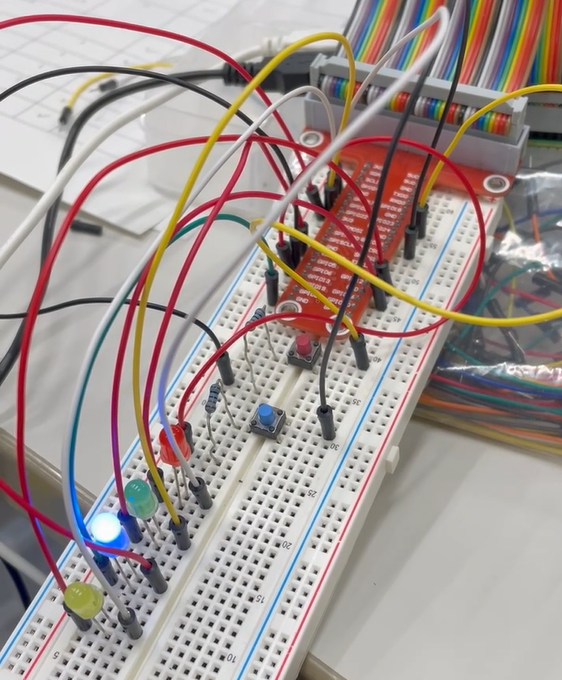
\includegraphics[width=0.5\textwidth]{result2-3.png} % 画像を挿入、幅をページ幅に合わせる
  \caption{スイッチを押した結果} % キャプションを追加
  \label{fig:result2-3} % ラベルを追加
\end{figure}

\subsection{考察}
複数のLEDを順番に点滅させることができたのは, while文内でledsという配列に対し0~3のインデックスを与えた
からだと考えられる. また, 課題2と同じように, スイッチが反応するのが0.5秒間隔だったのは, sleep.time(0.5)
のためであると考えられる. 

\section{課題2-4 単⼀ステッピングモータの制御}

\subsection{目的・概要}
Raspberry Pi を⽤いてステッピングモータの制御を⾏う. Raspberry Piとステッピングモータ1個を接続
し, ステッピングモータをユニポーラ1相励磁, 2相励磁, 1-2相励磁により正転, 逆転, 停⽌を⾏うコードを
作成して動作する.  

\subsection{必要な部品}

\subsubsection{課題2-1, 2-2と同じ部品}
Raspberry Pi 3 model B+, Micro SDカード
, HDMIケーブル, Micro USB電源ケーブル
, モニタ, USBキーボード, USBマウス
ブレッドボード, GPIOブレッドボード接続ケーブルは課題2-1, 2-2と同じものを使用する. 

\subsubsection{ステッピングモータ}
モータの各相(コイル)に,ある順序で励磁パルスを与えると⼀定⾓度回転する. 

\subsubsection{ステッピングモータ制御回路}
モータをあらかじめ設定した励磁⽅式に従って電流を流すように制御する. 

\subsubsection{2.1mm DCジャック}
USB DC5V to DC12V 昇圧ケーブルを接続し, モバイルバッテリーを使う. 

\subsubsection{USB DC5V to DC12V 昇圧ケーブル}
モバイルバッテリーとDCジャックを接続する. 

\subsubsection{モバイルバッテリー}
ELECOM社のEC-M01BKを使用した. 

\subsubsection{配線ケーブル}
オス-オスとメス-オスの両方を使用した. 


\subsection{実験方法}

表\ref{tab:tab2-4}のように, ステッピングモータとステッピングモータ制御回路を配置した. 
モバイルバッテリーをUSB DC5V to DC12V 昇圧ケーブルを用いて, DCジャックに接続した. 
このときの状況を, 図\ref{fig:raspi2-4}に示す. 

\begin{table}[H] % ここで[h]は表の位置をこの場所にすることを指定します
  \centering % 表を中央に配置
  \caption{回路の接続方法}
  \begin{tabular}{|c|c|} 
  \hline % 上の横線
  接続元 & 接続先  \\ \hline % 行の内容と行間の横線
  モータ制御回路 IN 1 & GPIO6    \\ \hline
  モータ制御回路 IN 2 & GPIO13   \\ \hline
  モータ制御回路 IN 3 & GPIO19   \\ \hline
  モータ制御回路 IN 4 & GPIO26   \\ \hline
  モータ制御回路 + & DCジャック + \\ \hline
  モータ制御回路 - & DCジャック - \\ \hline
  DCジャック -  & GND \\ \hline

  \end{tabular}
  \label{tab:tab2-4} % 表を参照するためのラベル
\end{table}

Raspberry Piによる1相励磁による正転, 逆転, 停⽌制御コード2-4-1.py, 2相励磁による正転, 逆転, 停⽌制御コード2-4-2.py, 
1-2相励磁による正転, 逆転, 停⽌制御コード2-4-3.py,を作成した. 
これらを, 図\ref{fig:2-4-1py}, 図\ref{fig:2-4-2py}, 図\ref{fig:2-4-3py}に示す.
その後, 2-4-1.py, 2-4-2.py, 2-4-3.py,をRaspberry Pi上で実行した. 

\begin{figure}[H] % 画像を挿入する環境を開始
  \centering
  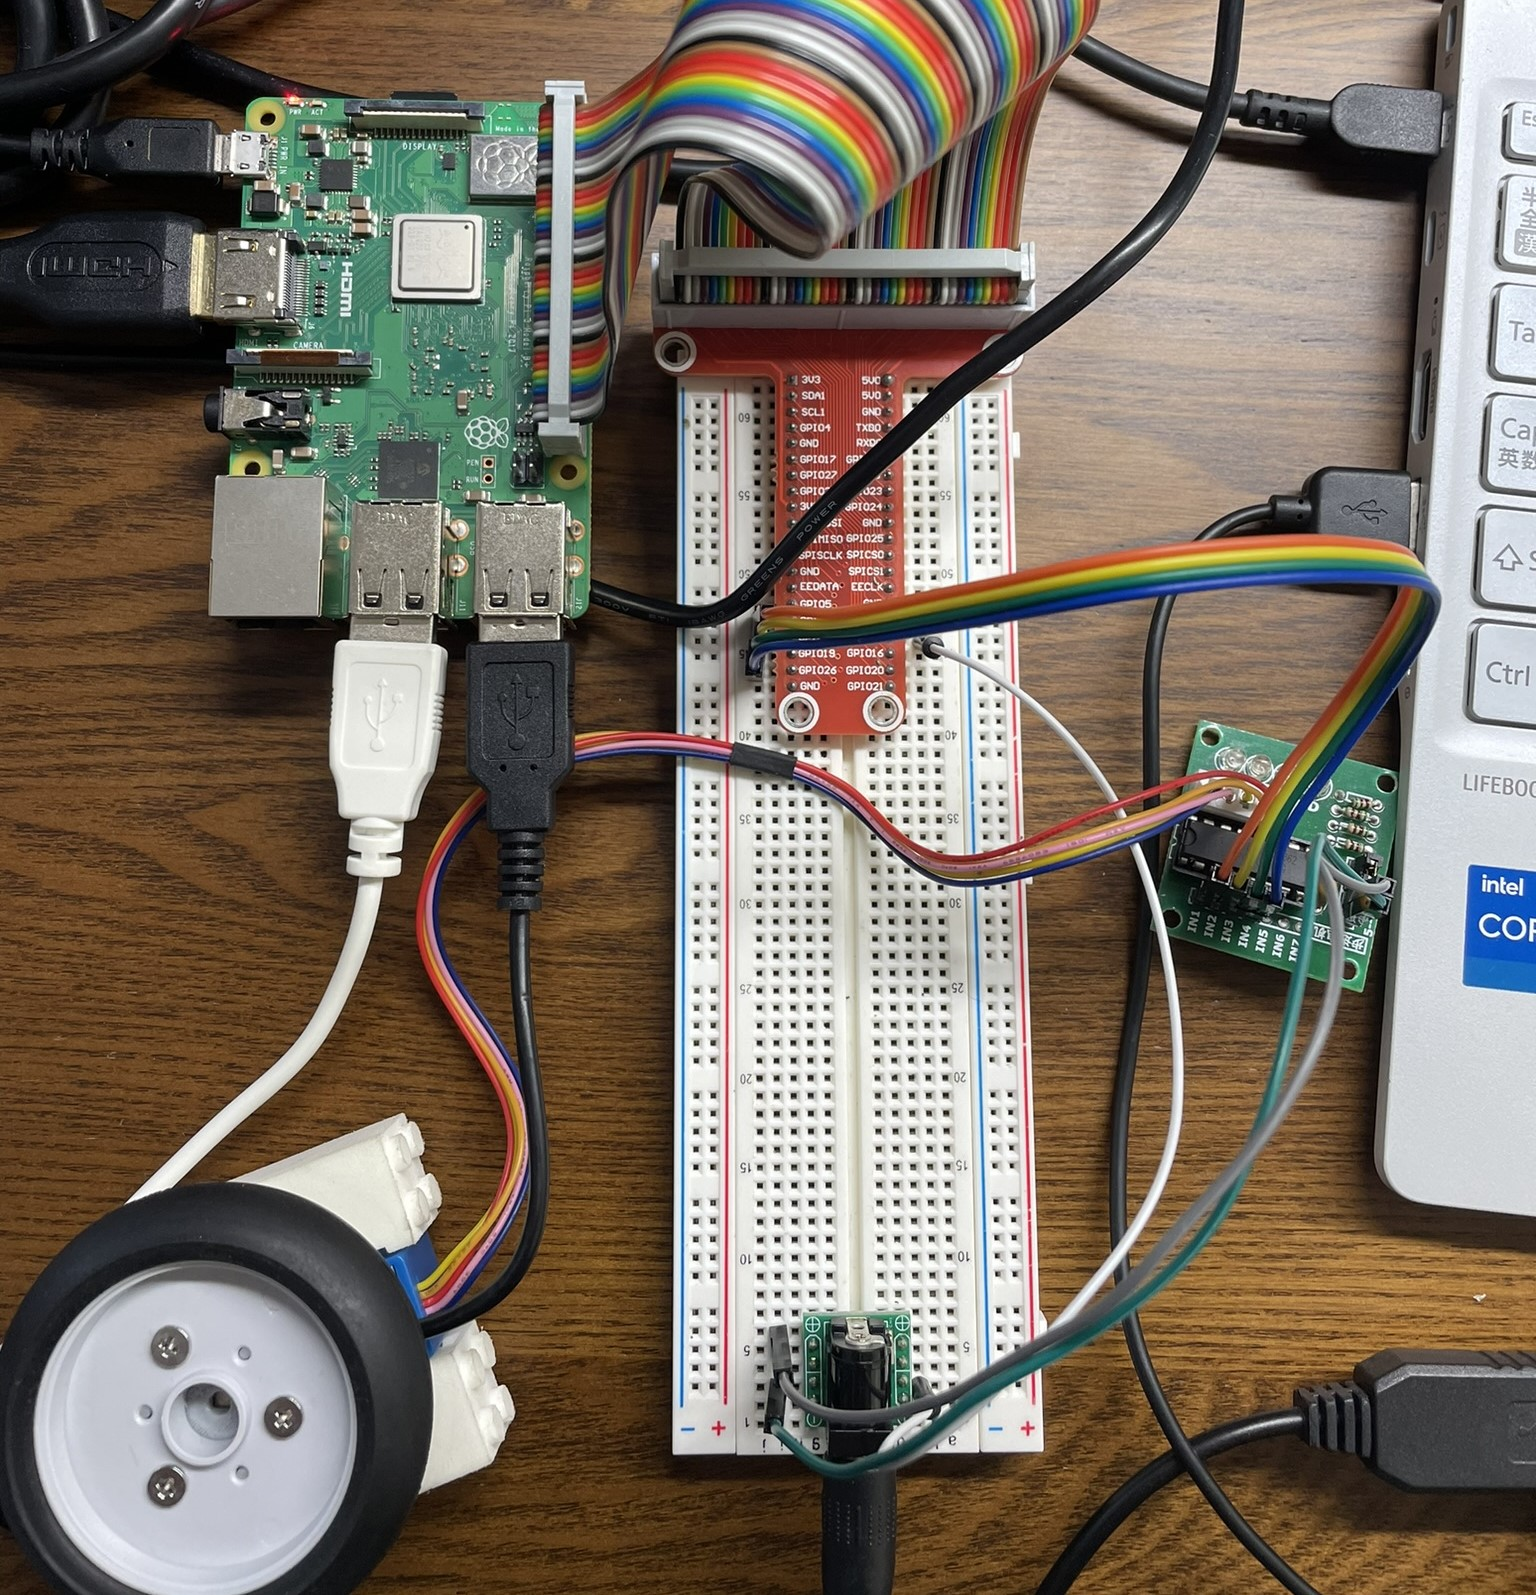
\includegraphics[width=0.5\textwidth]{raspi2-4.JPEG} % 画像を挿入、幅をページ幅に合わせる
  \caption{課題2-4の配線状況} % キャプションを追加
  \label{fig:raspi2-4} % ラベルを追加
\end{figure}

\begin{mdframed}
  \begin{verbatim}
    //省略

    # 1相励磁によるステッピングモータ運転
    while True:
        i = 0
        for j in range(0, 1000):   
            out_motor_pin(i)
            i += 1
            if i >= 4:
                i = 0 # ⼀周したら戻る
            # 乱調を避けるために少し待つ
            time.sleep(TIME_SLEEP)

        i = 3
        for j in range(0, 1000):   
            out_motor_pin(i)
            i -= 1
            if i <= -1:
                i = 3 # ⼀周したら戻る
            # 乱調を避けるために少し待つ
            time.sleep(TIME_SLEEP)

        for j in range(0, 1000):   
            out_motor_pin(i)

            # 乱調を避けるために少し待つ
            time.sleep(TIME_SLEEP) 	
  \end{verbatim}
  \end{mdframed}
  \begin{figure}[H]
  \caption{2-4-1.py}
  \label{fig:2-4-1py}
  \end{figure}



\begin{mdframed}
    \begin{verbatim}
      //省略
  
      # 逆回転で指定した2相を励磁する関数2
      def two_out_motor_pin2(pin_num):
          #1つ後ろのコイル
          pin_next = pin_num + 1
          if pin_next >= 4:
              pin_next -= 4
        
          for i in range(0, 4):
              if i == pin_num or i == pin_next:
                  motor_pins[i].on()
              else:
                  motor_pins[i].off()
            
      # 2相励磁によるステッピングモータ運転
      while True:
          i = 0
          for j in range(0, 1000):   
              two_out_motor_pin1(i)
              i += 1
              if i >= 4:
                  i = 0 # ⼀周したら戻る
              # 乱調を避けるために少し待つ
              time.sleep(TIME_SLEEP)
      
          i = 3
          for j in range(0, 1000):   
              two_out_motor_pin2(i)
              i -= 1
              if i <= -1:
                  i = 3 # ⼀周したら戻る
              # 乱調を避けるために少し待つ
              time.sleep(TIME_SLEEP)
      
          for j in range(0, 1000):   
              two_out_motor_pin1(i)
      
              # 乱調を避けるために少し待つ
              time.sleep(TIME_SLEEP) 	
    \end{verbatim}
    \end{mdframed}
    \begin{figure}[H]
    \caption{2-4-2.py}
    \label{fig:2-4-2py}
    \end{figure}

    

    \begin{mdframed}
      \begin{verbatim}
        //省略
    
        # 1, 2相励磁によるステッピングモータ運転
        while True:
            i = 0
            for j in range(0, 1000):
                if j%2==0:
                    out_motor_pin(i)
                else:
                    two_out_motor_pin1(i)
                    i += 1              
                if i >= 4:
                    i = 0 # ⼀周したら戻る
                # 乱調を避けるために少し待つ
                time.sleep(TIME_SLEEP)

            i = 3
            for j in range(0, 1000):   
                if j%2==0:
                    out_motor_pin(i)
                else:
                    two_out_motor_pin2(i) 
                    i -= 1
                if i <= -1:
                    i = 3 # ⼀周したら戻る
                # 乱調を避けるために少し待つ
                time.sleep(TIME_SLEEP)

            for j in range(0, 1000):   
                two_out_motor_pin1(i)

                # 乱調を避けるために少し待つ
                time.sleep(TIME_SLEEP)  	
      \end{verbatim}
      \end{mdframed}
      \begin{figure}[H]
      \caption{2-4-3.py}
      \label{fig:2-4-3py}
      \end{figure}    


\subsection{実験結果}
2-4-1.pyを実行すると, ステッピングモーターがある程度正転し, 逆転し, 停止し, 再び正転した. 

2-4-2.pyを実行したときも同様に, 正転, 逆転, 停止を繰り返した. 
また, 2-4-1.pyを実行したときよりも, 振動が小さかった. 

2-4-3.pyを実行したときも同様に, 正転, 逆転, 停止したが, 回転速度は2-4-1.py, 2-4-2.pyを実行したときよりも遅かった. 

また, TIME SLEEPを0.2に設定し実行したところ, 2-4-1.pyではランプが1つずつつき, 
2-4-2.pyではランプが2つずつつき, 2-4-3.pyではランプが1つつくと2つつくを繰り返した. 

\subsection{考察}
2相が1相に対して振動が小さかったのは, ⼆つの相を同時に吸収するからだと考えられる. 

1-2 相励磁⽅式の回転速度が遅かったことに疑問を抱いたので, これについて調べた. 1-2 相励磁⽅式は, 1 相励磁⽅式と
2相励磁⽅式とを交互に⾏うことで回転磁界を作り, 回転⼦を回転する⽅式である. 
SW1 から SW4の各コイルは, 表\ref{tab:motor1-2}に示すように変化する. 
1相励磁時から2相励磁に切り替わると1/4ピッチずれた状態になり, 
再び1相励磁になるとずれが1/2ピッチになる. 
このように, 1-2 相励磁⽅式は1 相励磁⽅式や2相励磁⽅式に対してステップ角が半分になるので, 回転速度が遅くなる. 
(ana-dig, 2024)


\begin{table}[H] % ここで[h]は表の位置をこの場所にすることを指定します
  \centering % 表を中央に配置
  \caption{1-2 相励磁⽅式の各相の入力状態}
  \begin{tabular}{|c|c|c|c|c|c|c|c|c|} 
  \hline % 上の横線
  SW / step & 1 & 2 & 3 & 4 & 5 & 6 & 7 & 8\\ \hline % 行の内容と行間の横線
  SW1 & 1 & 1 & 1 & 0 & 0 & 0 & 0 & 0\\ \hline
  SW2 & 0 & 0 & 1 & 1 & 1 & 0 & 0 & 0\\ \hline
  SW3 & 0 & 0 & 0 & 0 & 1 & 1 & 1 & 0\\ \hline
  SW4 & 1 & 0 & 0 & 0 & 0 & 0 & 1 & 1\\ \hline

  \end{tabular}
  \label{tab:motor1-2} % 表を参照するためのラベル
\end{table}

本来今回の実験では, USB DC5V to DC12V 昇圧ケーブルとモバイルバッテリーは使わないはずであったが, 指導書を読み間違えてしまったことにより, 
課題2-5のようにこれらを使用して回路を作成してしまった. 幸い大きな問題はなかったが, 今後は間違えないように気を付けたい.


\section{課題2-5 複数ステッピングモータの制御}

\subsection{目的・概要}
Raspberry Pi を⽤いて,複数の押しボタンスイッチからの⼊⼒に基づき,複数のステッピングモータを制御
する.

\subsection{必要な部品}

\subsubsection{課題2-1, 2-2, 2-4と同じ部品}
Raspberry Pi 3 model B+, Micro SDカード
, HDMIケーブル, Micro USB電源ケーブル
, モニタ, USBキーボード, USBマウス
ブレッドボード, GPIOブレッドボード接続ケーブル, 抵抗内蔵LED, 押しボタンスイッチ, 抵抗
, 配線ケーブル, ステッピングモータ, ステッピングモータ制御回路, 
2.1mm DCジャック,  USB DC5V to DC12V 昇圧ケーブル, 
モバイルバッテリーは課題2-1, 2-2, 2-4と同じものを使用する. 


\subsection{実験方法}

表\ref{tab:tab2-5}のように, ステッピングモータ, テッピングモータ制御回路, 抵抗, 押しボタンスイッチを配置した.
このときの状況を, 図\ref{fig:raspi2-5}に示す. 

\begin{table}[H] % ここで[h]は表の位置をこの場所にすることを指定します
  \centering % 表を中央に配置
  \caption{回路の接続方法}
  \begin{tabular}{|c|c|c|} 
  \hline % 上の横線
  接続する部品 & 接続1 & 接続2 \\ \hline % 行の内容と行間の横線
  抵抗とSWITCH1 & GPIO5 & GND \\ \hline
  抵抗とSWITCH2 & GPIO23 & GND \\ \hline
  モータ制御回路1 IN 1 & GPIO6 &   \\ \hline
  モータ制御回路1 IN 2 & GPIO13 &  \\ \hline
  モータ制御回路1 IN 3 & GPIO19 &  \\ \hline
  モータ制御回路1 IN 4 & GPIO26 &  \\ \hline
  モータ制御回路1 + & DCジャック + & \\ \hline
  モータ制御回路1 - & DCジャック - & \\ \hline
  モータ制御回路2 IN 1 & GPIO4 &   \\ \hline
  モータ制御回路2 IN 2 & GPIO17 &  \\ \hline
  モータ制御回路2 IN 3 & GPIO27 &  \\ \hline
  モータ制御回路2 IN 4 & GPIO22 &  \\ \hline
  モータ制御回路2 + & DCジャック + & \\ \hline
  モータ制御回路2 - & DCジャック - & \\ \hline
  DCジャック -  & GND & \\ \hline

  \end{tabular}
  \label{tab:tab2-5} % 表を参照するためのラベル
\end{table}

複数の押しボタンスイッチからの⼊⼒に基づき, 複数のステッピングモータを制御するコード2-5.pyを作成した. 

これを, 図\ref{fig:2-5py}に示す.
その後, 2-5.pyをRaspberry Pi上で実行し, 二つのスイッチを押したり離したりした. 

\begin{figure}[H] % 画像を挿入する環境を開始
  \centering
  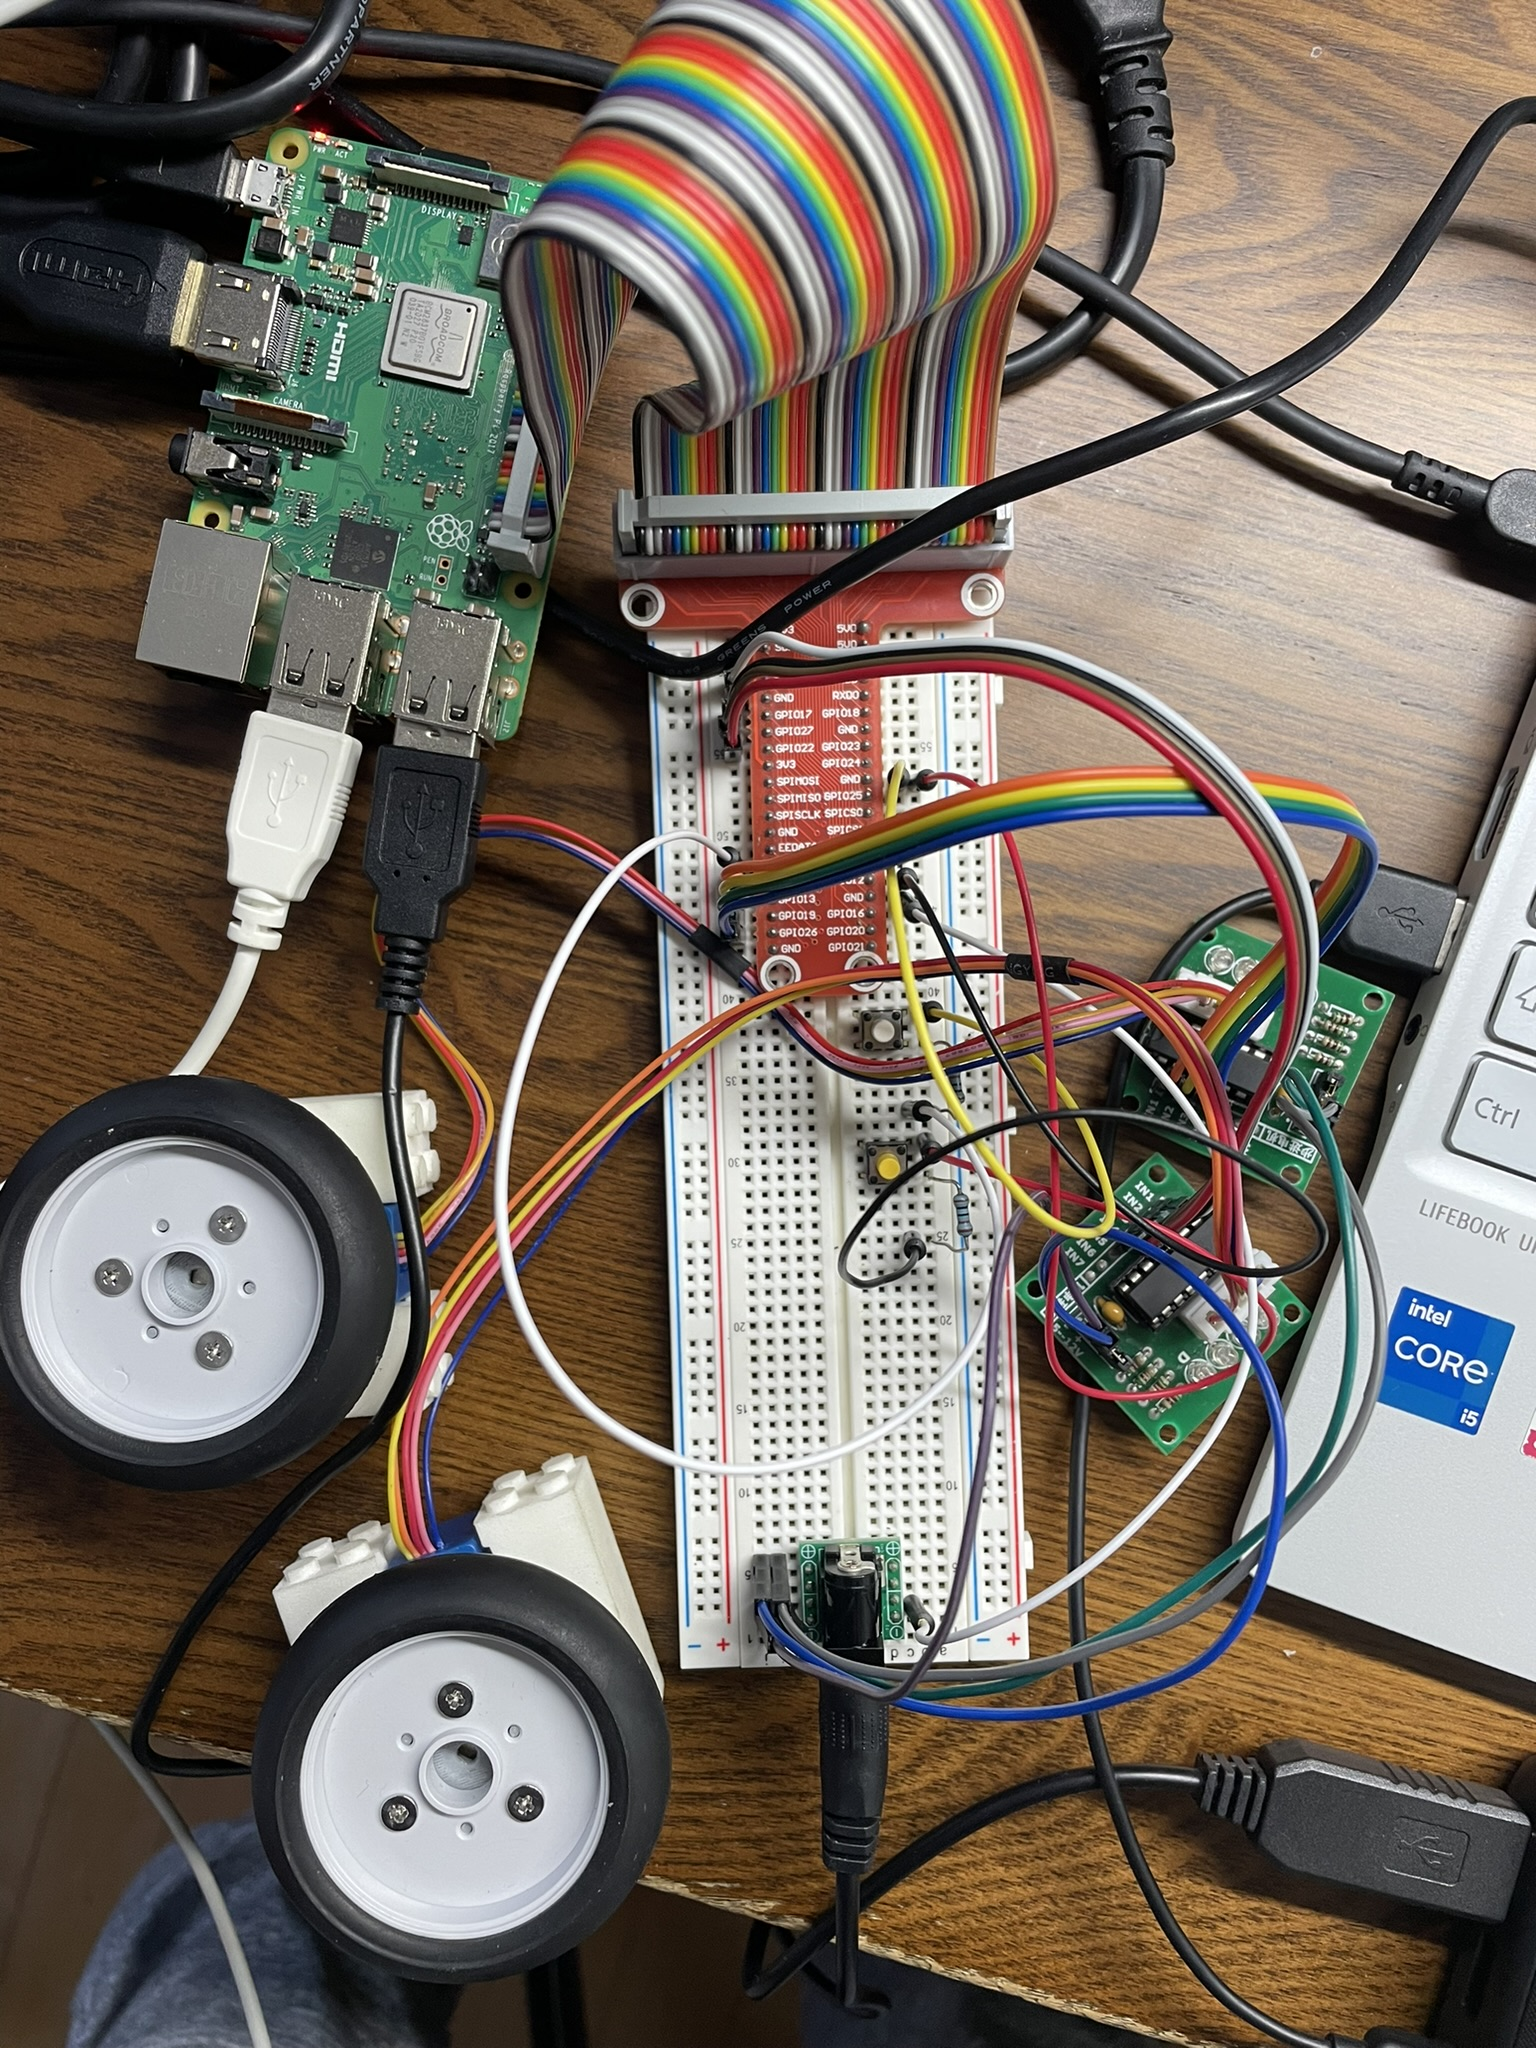
\includegraphics[width=0.5\textwidth]{raspi2-5.JPEG} % 画像を挿入、幅をページ幅に合わせる
  \caption{課題2-5の配線状況} % キャプションを追加
  \label{fig:raspi2-5} % ラベルを追加
\end{figure}

\begin{mdframed}
  \begin{verbatim}
    //省略

    isStopped=False
    isReversed=False
    
    # 1相励磁によるステッピングモータ運転
    i = 0 #モーター1
    j = 0 #モーター2
    while True:
        # スイッチ1接続端⼦の状態読み取り
        if switch1.value == 1:
            if(isStopped == False):
                isStopped = True #止める判定
            else:
                isStopped = False #止める判定        
            print("Switch1 on")
            time.sleep(1)
    
        # スイッチ2接続端⼦の状態読み取り    
        if switch2.value == 1: 
            if(isReversed == False):
                isReversed = True #逆判定
            else:
                isReversed = False #逆判定    
            print("Switch2 on")
            time.sleep(1)
    
        if isStopped == True:
            time.sleep(1)
        else:
            i += 1
            if i >= 4:
                i = 0
    
            if isReversed == True:
                j-=1
                if j <= -1:
                    j = 3
            else:
                j+=1
                if j >= 4:
                    j = 0
            out_motor1_pin(i)
            out_motor2_pin(j)
            # 乱調を避けるために少し待つ
            time.sleep(TIME_SLEEP)	
  \end{verbatim}
  \end{mdframed}
  \begin{figure}[H]
  \caption{2-5.py}
  \label{fig:2-5py}
  \end{figure}


\subsection{実験結果}
2-5.pyを実行すると, 2つのステッピングモータが同じ方向に回転した. 
スイッチ1を押すと, 両方のモータが停止した. 再びスイッチ1を押すと, 両方のモータが回転した. 
スイッチ2を押すと, 片方のモータが逆回転した. 再びスイッチ2を押すと, モータの回転方向が戻った. 


\subsection{考察}
停止と逆回転の実装は, 課題2-3と同じ原理である. isStopped, isReversedのbooleanの値を使い, 
ステッピングモータの回転を制御している. この方法が直感的に理解しやすいと考えた.  


\section{まとめ}

\subsection{実験を通して分かったこと}
Raspberry Piを用いたLED, スイッチ, ステッピングモータの制御の方法を理解した. 

\subsection{工夫したこと}
実験で行ったことについて逐一メモや写真に記録を残し, 後から確認しやすいようにした.

\subsection{反省点}
課題2-4で仕様書を読み間違えてしまった. 仕様書では, Raspberry Pi の5V出力を使うはずだったが, 
課題2-5と同様にモバイルバッテリーを使ってしまった. 今回の実験では大きな問題にならなかったが, 
今後はこのようなミスをなくしたい. 


\begin{thebibliography}{99} % 最大ラベル幅を99に設定
    
  \bibitem{lamport1994latex}
  PassMark: 
  \emph{ステッピングモータの動作原理}. \\
  \verb|https://ana-dig.com/stepper-motor1/|  2024.

\end{thebibliography}


\end{document}